\section{Společně odvedená práce}

\label{sec:team_work}

\subsection{Důvod vybrání tématu týmem}
Téma Rezervačního systému se nám líbilo nejvíce. Zaujala nás rada od zkušeného programátora, který podotkl, že rezervačních systému je na trhu nedostatek. Je jistě užitečnější vytvořit program, který se někomu možná bude jednou hodit.

\subsection{Analýza uživatele - co uživatel dělá v reálném životě, jaký je\\
proces/činnost, kterou vykonává a kde by mu příp. vhodný SW mohl
pomoci}
Každý člen našeho týmu si zvolil uživatele s jiným zaměřením.
Námi vybraná skupina uživatelů jsou poskytovatelé služeb. Každý z nich má v nabídce paletu služeb, které poskytuje svým zákazníkům.
Problém ale nastával při domlouvání realizace samotné služby. Nejčastěji se jednalo o chybu "v lidském faktoru". Na recepci seděl člověk a ten rezervace spisoval.
Rezervace byly špatně poznačené nebo poskytovatelé zapomněli informovat zákazníky o zrušení apod.
V případě online rezervačního systému by byla rezervace ponechána klientovi, čímž by se mohlo předejít už nahoře zmíněným chybám lidského faktoru.
Systém by rovněž informoval zákazníka obratem o stavu rezervace a uměl by taky informovat o nastávající rezervaci apod.


\subsection{Potřeby uživatele - co je cílem činnosti, čeho chce dosáhnout}
V případe poskytovatele služeb, každý z nich potřeboval:
\begin{itemize}
    \item možnost vytvoření rezervace pro jimi nabízené služby
    \item minimalizovat potřebu interakce s klienty - časově náročné
    \item potvrzení a informování zákazníků o vytvořené rezervaci
    \item editace rezervace
    \item jednoduchost systému
\end{itemize}

\subsection{Shrnutí současných řešení a výsledné pro a proti, inspirace, nápady}
V současné době se na trhu vyskytuje nedostatek služeb, které nabízí nějakou formu rezervačního systému. Rezervační systém typu
"papír a pero" nám sloužil jako šablona dat, která byla zapotřebí při vytváření systému.
Webové aplikace, které již na trhu existují jsou sice jednoduché na používání, ale pro klienty. Pro poskytovatele služeb se jednalo častokrát
o neefektivní a drahé řešení ve formě SW "šitého na míru" či webová aplikace, která má až zbytečně moc nepotřebné funkcionality. T.j
poskytovatel služeb zbytečně platil za něco, co nevyužívá.


\subsection{Návrh zadání - co má nové řešení zlepšit, co uživateli umožní, v čem
mu konkrétně pomůže, co uživateli konkrétně přinese, co má být
konkrétním výstupem, jak má vypadat nový uživatelský proces}

Při vytváření makety jsme se inspirovali již existujícími aplikacemi zmíněných v individuálních řešeních u jednotlivých členů týmu.
Při ladění jsme se drželi programátorských taktik KISS. Snažili jsme se dát uživatelům, co nejméně možností ztratit se v rozhraní.
T.j. naše řešení obsahuje co nejméně prvků, se kterými mohou interagovat.
Stačila nám základní funkcionalita, tedy vytváření a editace rezervací.
Zároveň jsme přihlédli na způsob, jak připojit aplikaci k již existující stránce poskytovatele. Věříme totiž, že internetová
stránka je v 21. století nutností a tím pádem jsme se rozhodli pro jednoduché připojení stránky s aplikací ve formě pluginu.
Tedy na stránce bude odkaz na samotnou aplikaci ve formě tlačítka nebo jiného hypertextového odkazu, která bude běžet na stejném
serveru, jako stránka poskytovatele. Jednalo by se tedy o nejminimalističtější řešení pro webovou aplikaci a tím pádem by bylo ve
výsledku potřebné minimum pro samotnou rezervační aplikaci

\newpage
\begin{figure}[h]
    \centering
    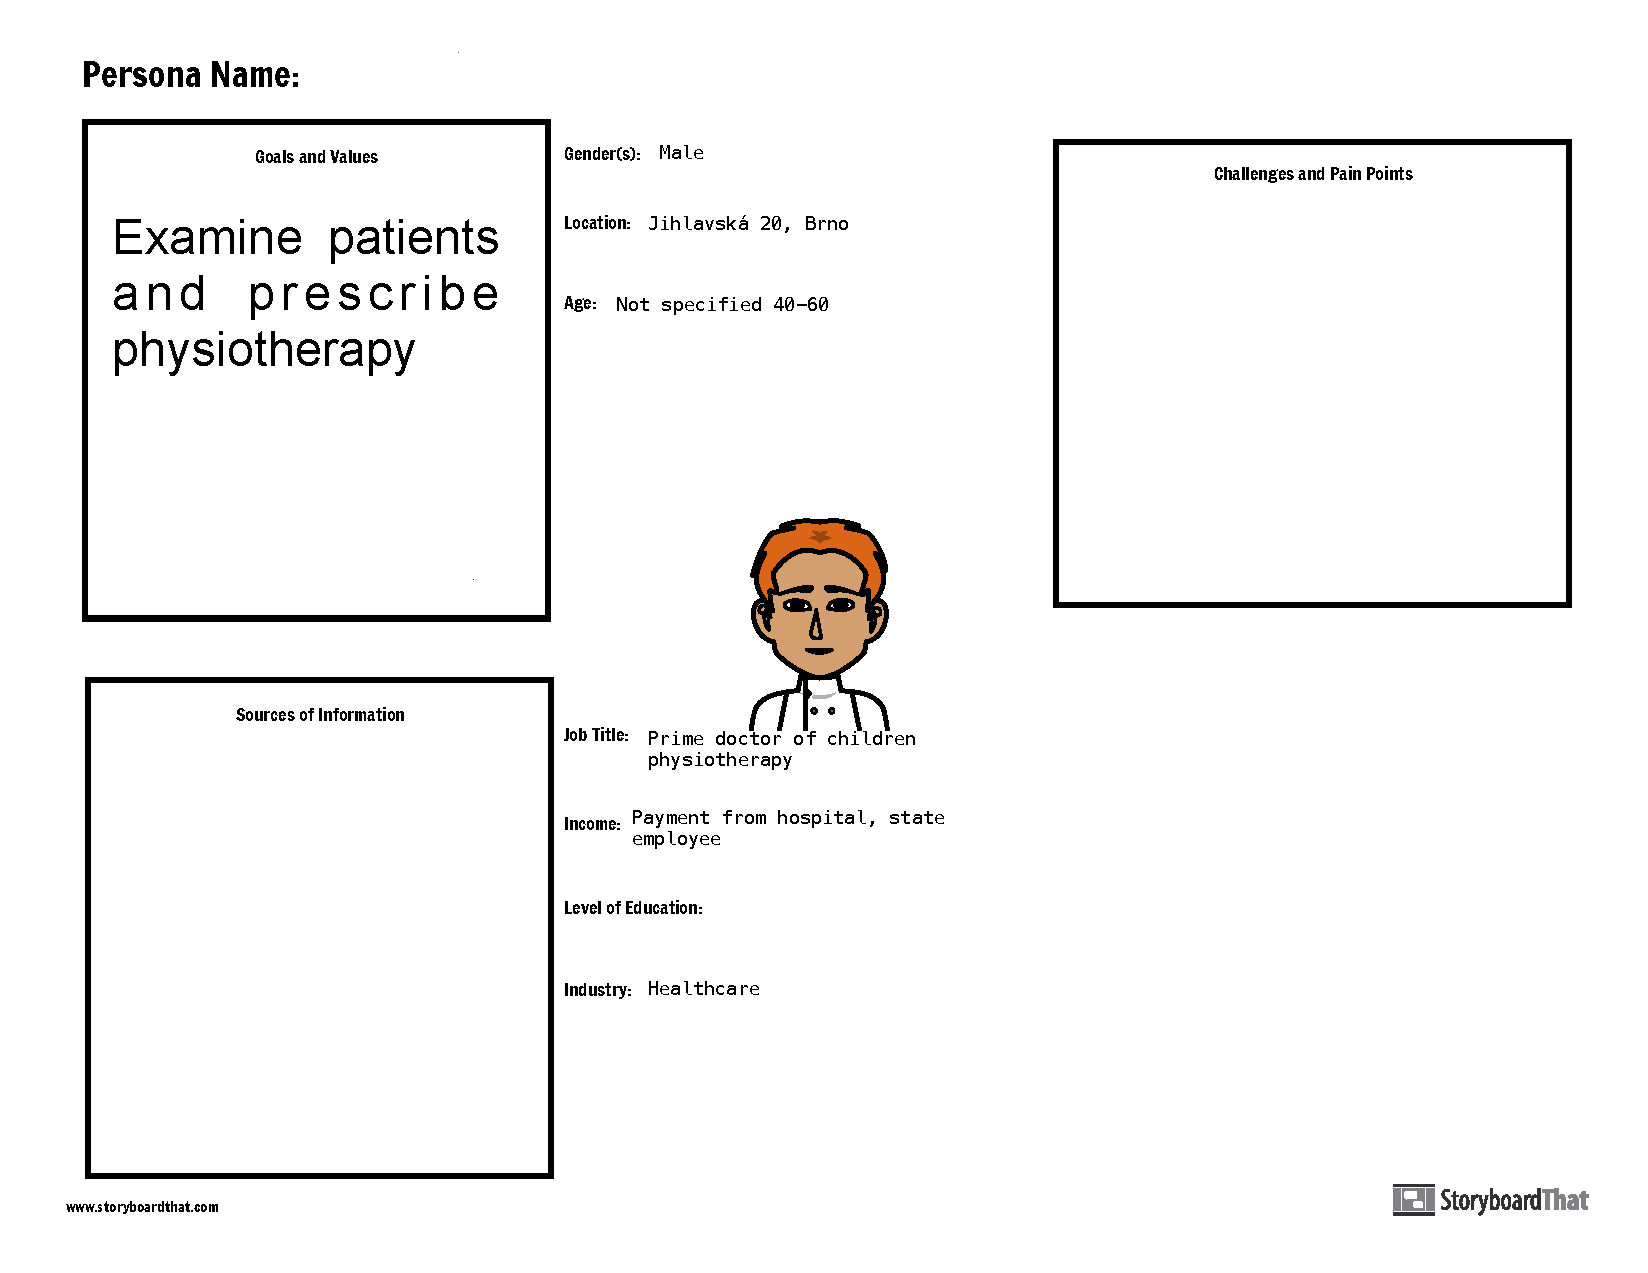
\includegraphics[width=1.4\textwidth, angle=270]{doc/latex/fig/vlado/Persona_Worksheets_PDF_dragged.pdf}
    \caption{Doktor}
    \label{fig:pers_doctor}
\end{figure}

\begin{figure}[h]
    \centering
    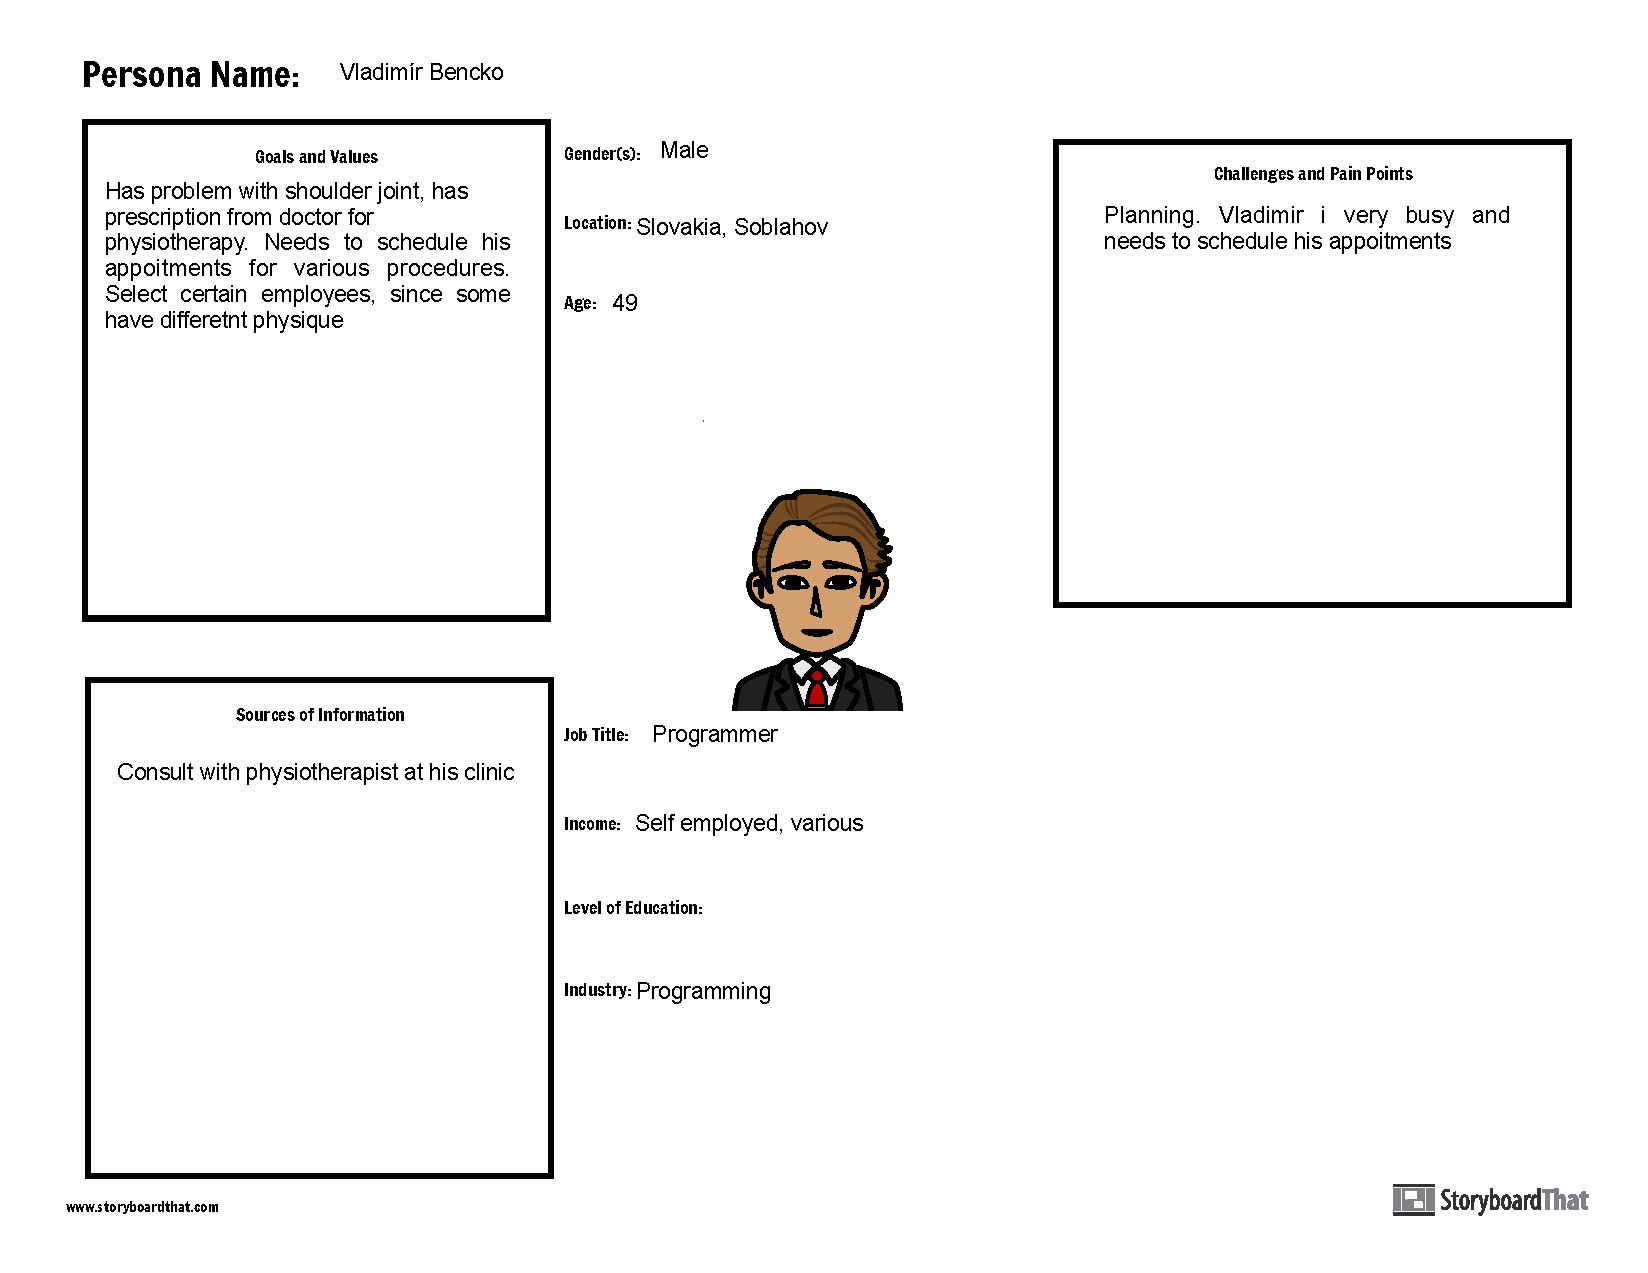
\includegraphics[width=1.4\textwidth, angle=270]{doc/latex/fig/vlado/Persona_Worksheets_PDF_dragged_2.pdf}
    \caption{Pacient}
    \label{fig:pers_patient}
\end{figure}

\begin{figure}[h]
    \centering
    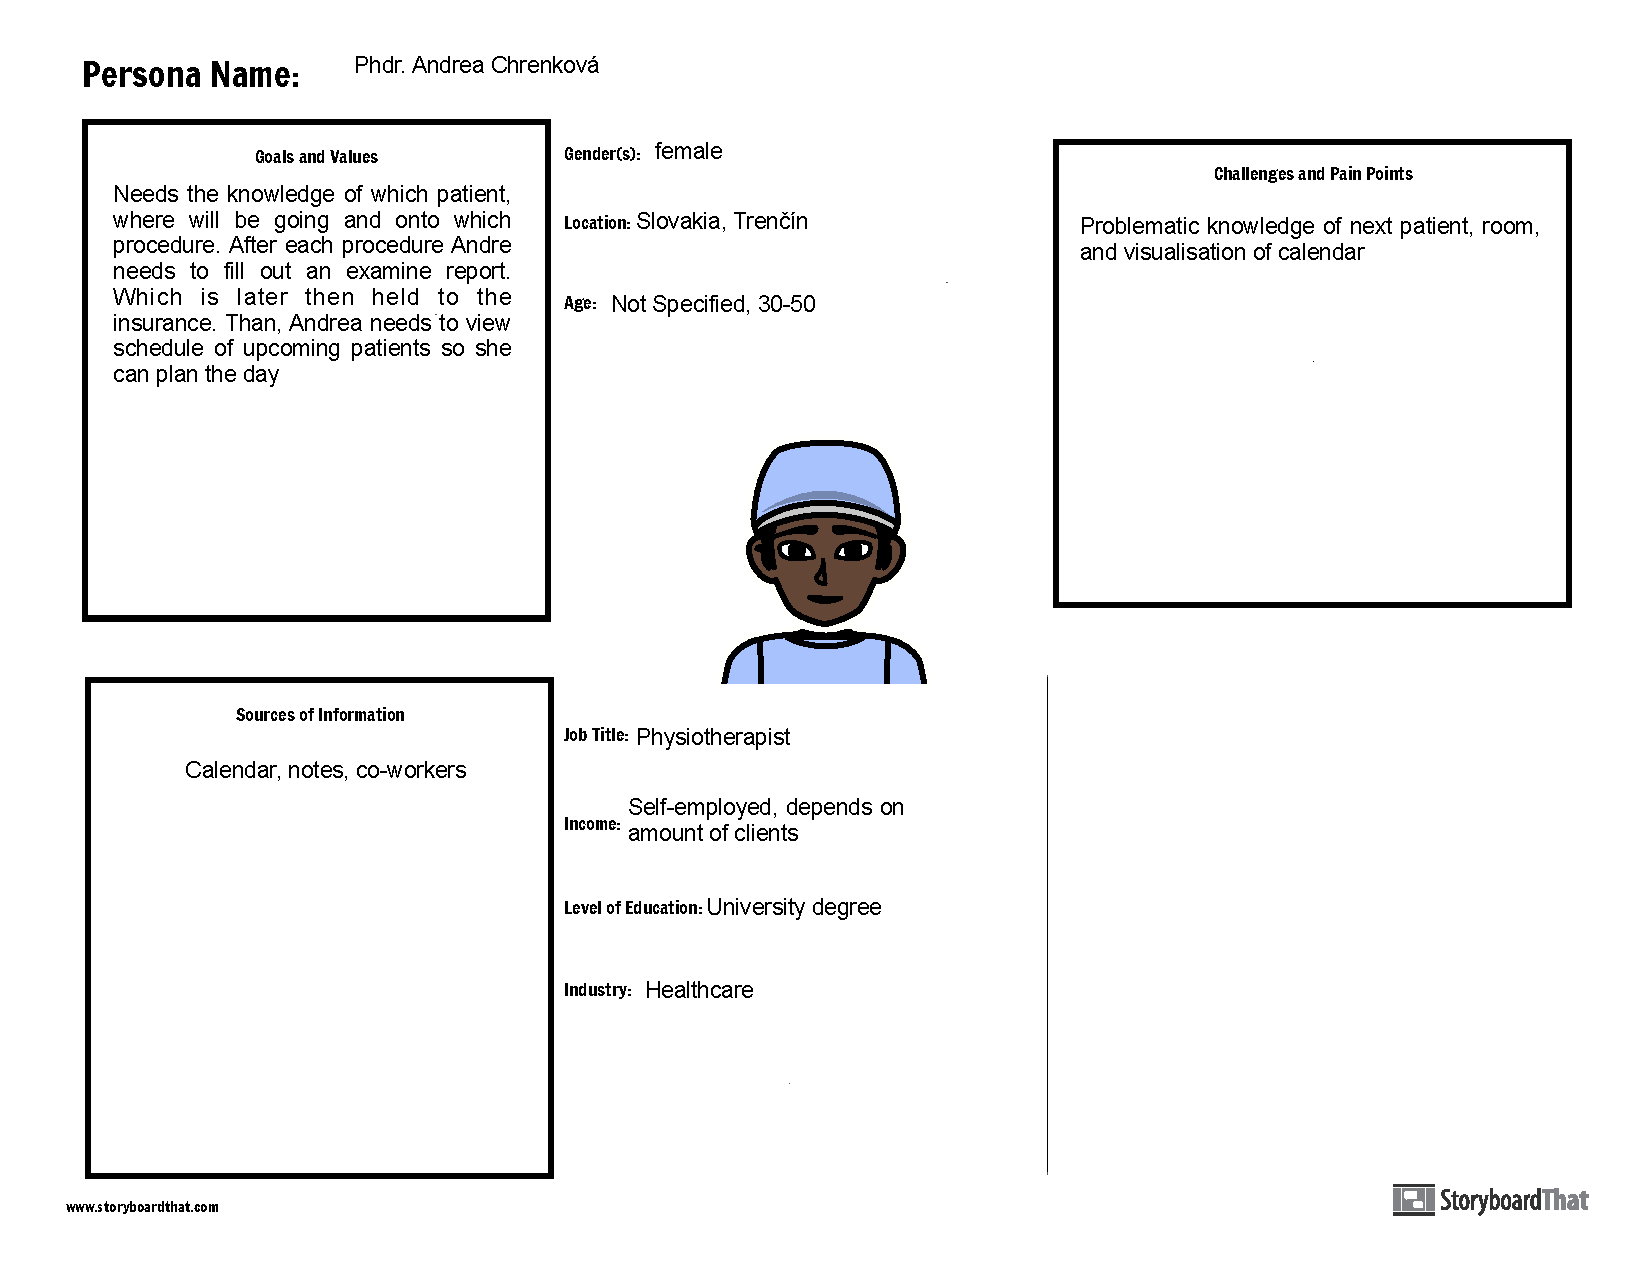
\includegraphics[width=1.4\textwidth, angle=270]{doc/latex/fig/vlado/Persona_Worksheets_PDF_dragged_3.pdf}
    \caption{Fyzioterapeut}
    \label{fig:pers_physio}
\end{figure}
\newpage



\subsection{Návrh řešení (předběžný) - nákresy vlastního řešení, datový model
    (datové struktury), popis API.}
Máme několik nápadu na popis API. Zatím jediný realizovaný způsob byl založen na komunikaci se serverem, který ukládá rezervace a posílá seznamy rezervací.
Zatím jsme kód nechali běžet\\ na bezplatném webhostingu Webzdarma.cz. Rezervace se dá na server poslat například pomocí \begin{quote}
    \href{https://iturezervacnisystem.wz.cz/index.php?jmeno=Vit}{https://iturezervacnisystem.wz.cz/index.php?jmeno=Vit}
\end{quote}. Server přijme atributy nazvané jmeno (viz. ukázka), den, mesic, rok, od, do, prijmeni, email, telefon, komentar, kategorie (kategorie služby jako masáže, sauny apod.) a specifikace (např. masáž obličeje). Pomocí příkazu nejblizsi=true lze zjistit nejbližší termíny. Příkaz rezervaceDanehoDne=true vypíše rezervace podle zvolených atributů den, měsíc a rok. Data vypisuje v formátu JSON. Technologii XML jsme použili pro načítání seznamu aktuálně nabízených služeb. Finální backend a API nakonec se vylepšila a začala nabízet více služeb pro práci s daty.

\newpage

\subsection{Testovnie aplikacie} \label{client_testing}

\subsubsection{Testovanie rozhrania pre klienta}
Testování proběhlo na dvou kamarádech z internátu, oba dva s problémy s páteří. \\
Testované prěbehlo vyzkoušením rozhraní.\\
Kvalita programu byla oproti referencnímu řesení snížena, avšak testovacím subjektům sa nelíbila minimalitičnost stránky.
Funkcionalita oproti referenčnímu řešení byla včak zachována.


Testovaná osoba 1

Záznam:
\textit{"Jednoduché, možno až moc. Pekne potriedené, mohlo by byť viac farebné. Zvolil som si masáž, prečo nie, po kliknutí sa
mi zobrazia viaceré možnosti,
dobrý nápad. Výber zamestnanca ... Výber dátumu. Prehľad dátumov je pekne spravený, zoradenie pod seba mi vizuálne
dobre oddeluje dátumy. Vyplnenie
osobných údajov ... mǒže byť. Aj komentár po vyplnení, fajn."}

Závěr:
\textit{"Viem o čo ste sa pokúšali, vyzerá to byť veľmi jednoduché. Mohlo by byť viac farebné. Ale objednať cez to sa dá.
Nie je to hrozné, nie je to výborné. Stačí to."}


Testovaná osoba 2

Záznam:
\textit{"Stránka na prvý pohľad mi príde minimalistická, základ. Farebná schéma nie je pekná ale postačujúca. Vyberte si službu
... biolampa. Vyberte si zaměstnance ...
tak isto ako predtým, proste obyčajné, biele, jednoduché ale prehľadné, nestratím sa v tom. Vyberte si datum, a tak,
dajme tomu utorok o deviatej ráno.
Tak isto ako predtým, úplne jednoduché.
Vyplnte své údaje, napíšem nejaké testovacie údaje. Odoslať."}

Závěr:
\textit{"Celkom v pohode. Jediné čo by osm dodal je, že mi to príde veľmi jednoduché, stránka je nezáživná a všetko je príliš
minimalistické."}

\newpage

\section{Sreenshoty z aplikacie}

\subsubsection{Rozhraní pro klienta}

\begin{figure}[h]
    \begin{subfigure}{.5\textwidth}
        \centering
        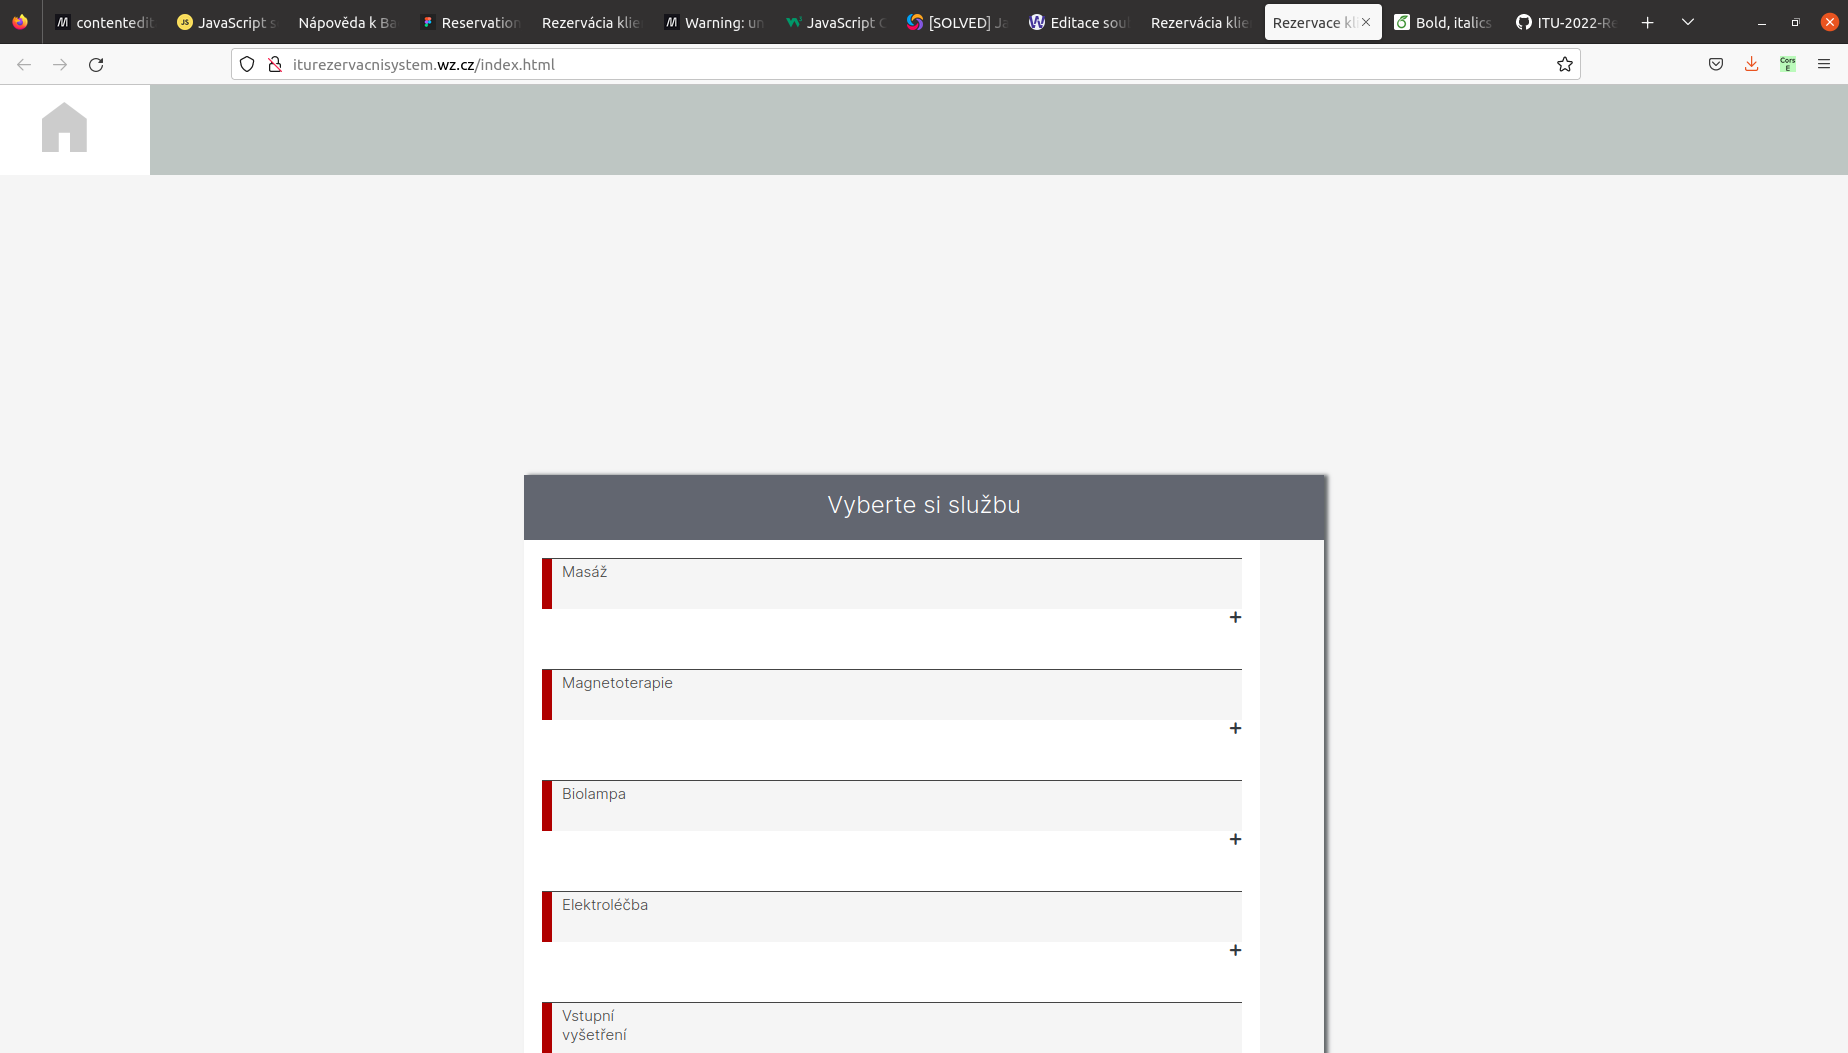
\includegraphics[width=.8\linewidth]{doc/latex/fig/implementation/client/step1.png}
        \caption{}
        \label{fig:step1}
    \end{subfigure}
    \begin{subfigure}{.5\textwidth}
        \centering
        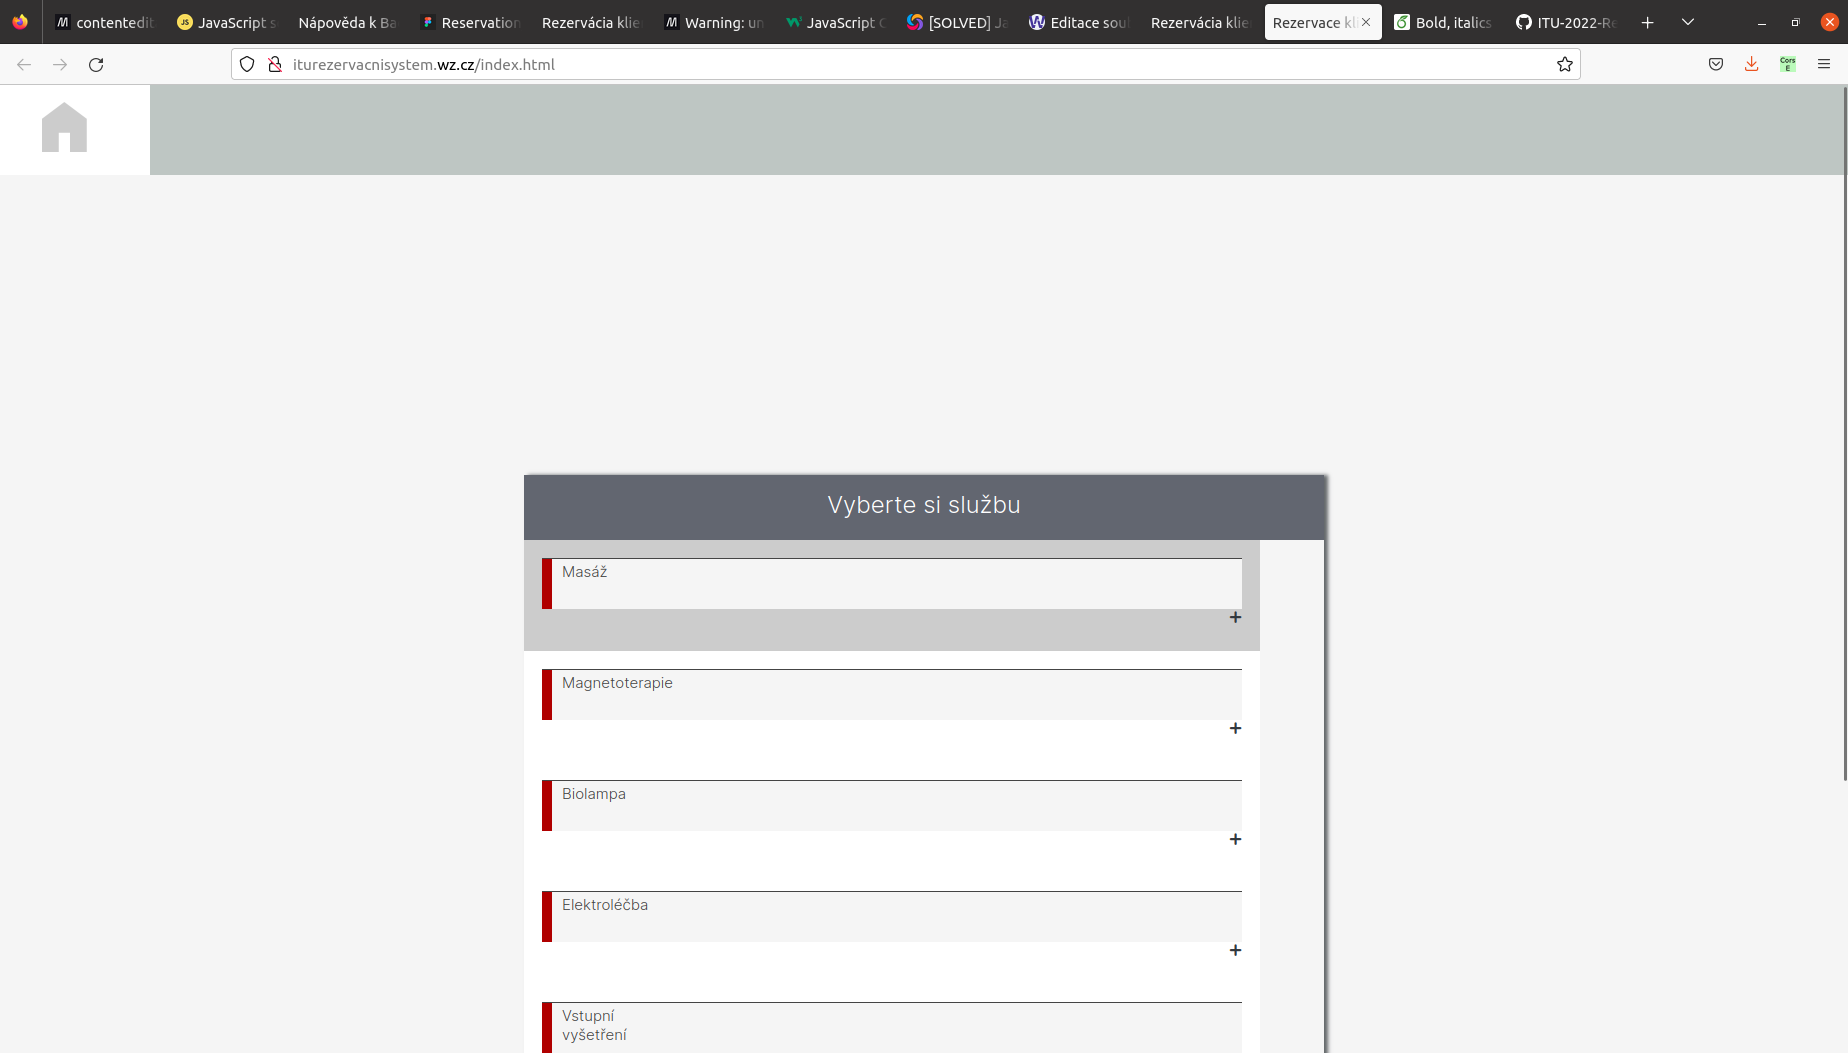
\includegraphics[width=.8\linewidth]{doc/latex/fig/implementation/client/step2.png}
        \label{fig:steps1}
    \end{subfigure}
\end{figure}

\begin{figure}[h]
    \begin{subfigure}{.5\textwidth}
        \centering
        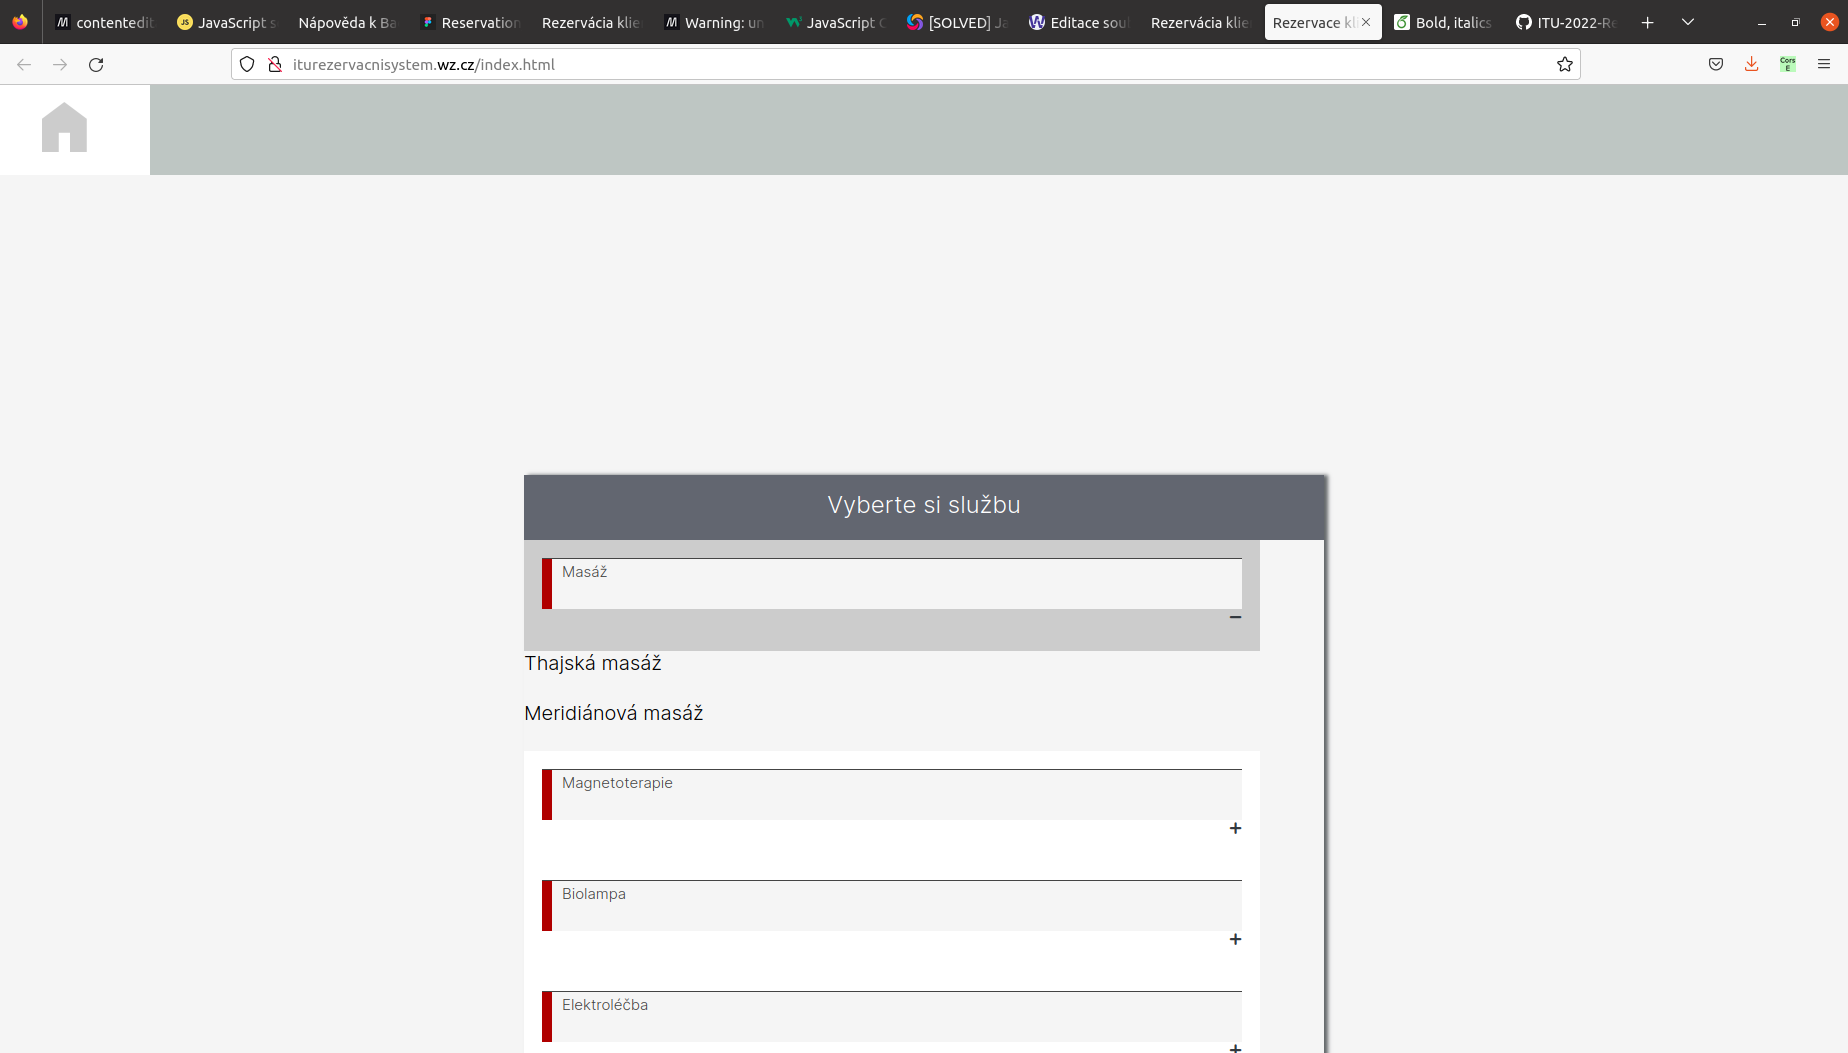
\includegraphics[width=.8\linewidth]{doc/latex/fig/implementation/client/step3.png}
        \caption{}
        \label{fig:step1}
    \end{subfigure}
    \begin{subfigure}{.5\textwidth}
        \centering
        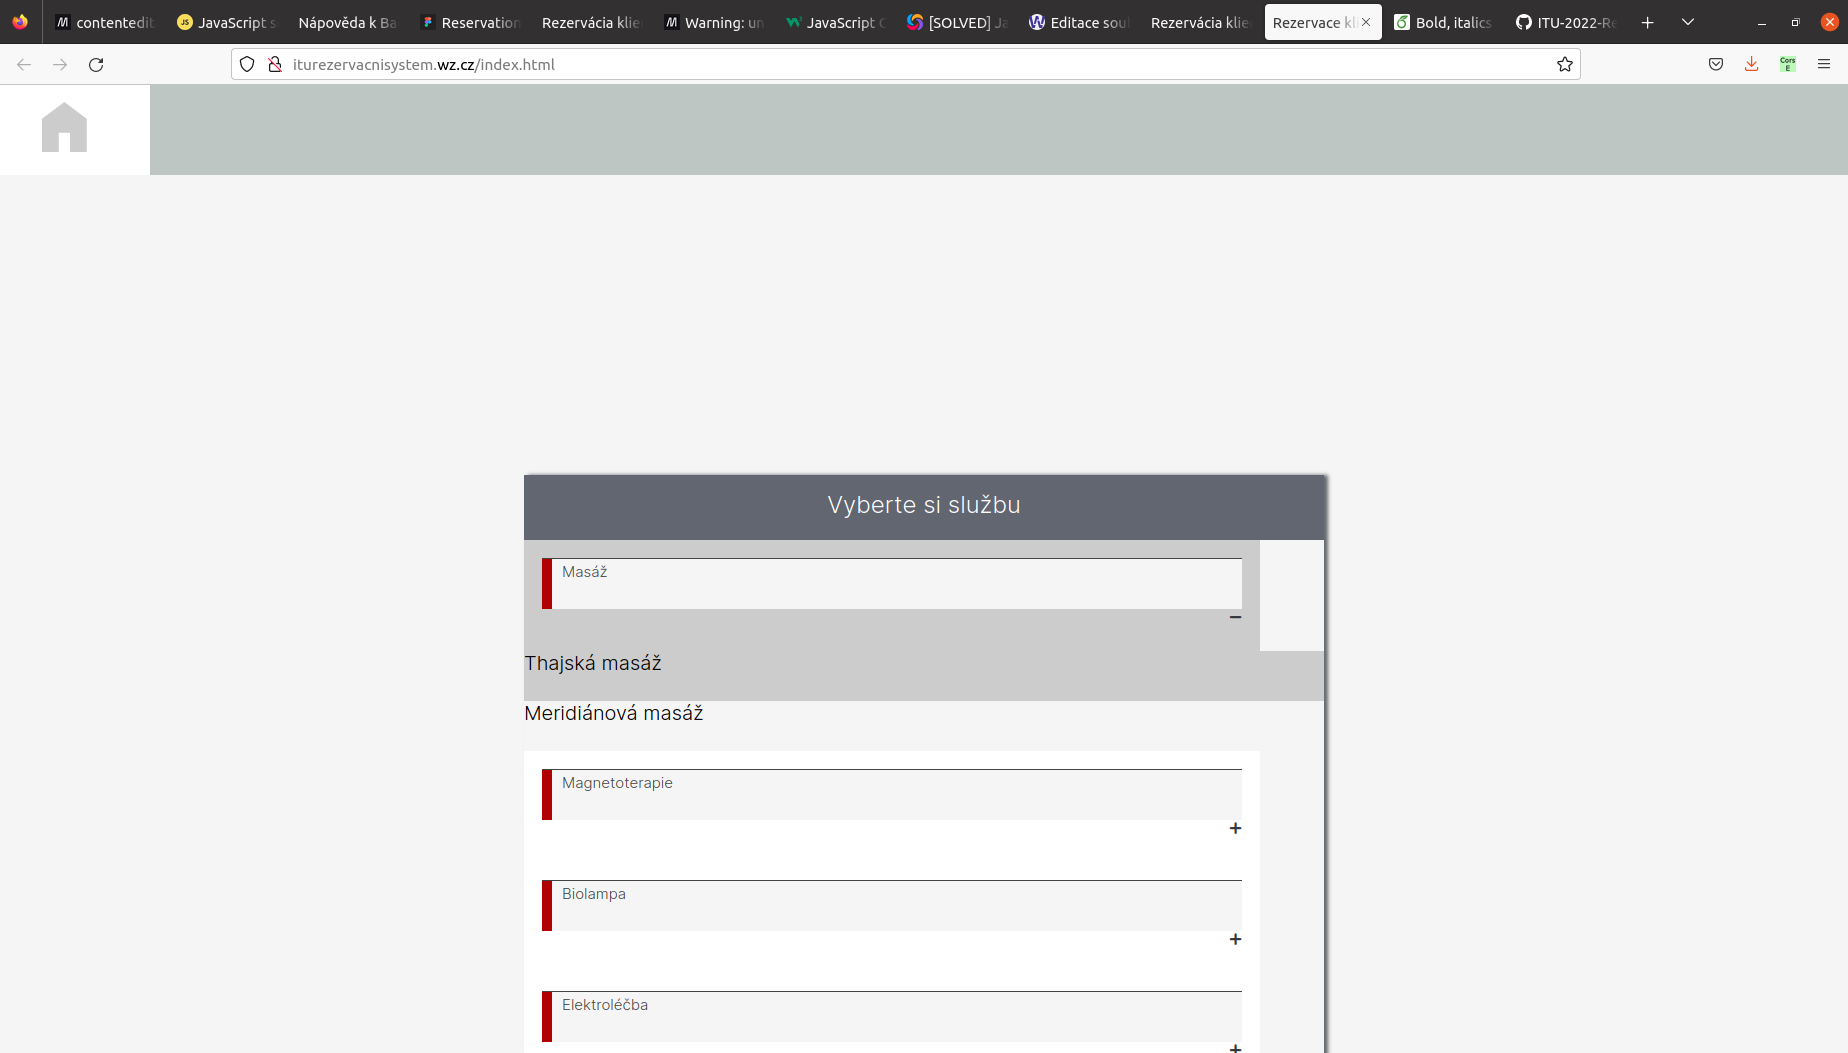
\includegraphics[width=.8\linewidth]{doc/latex/fig/implementation/client/step4.png}
        \caption{}
        \label{fig:step2}
    \end{subfigure}
    \label{fig:steps2}
\end{figure}

\begin{figure}[h]
    \begin{subfigure}{.5\textwidth}
        \centering
        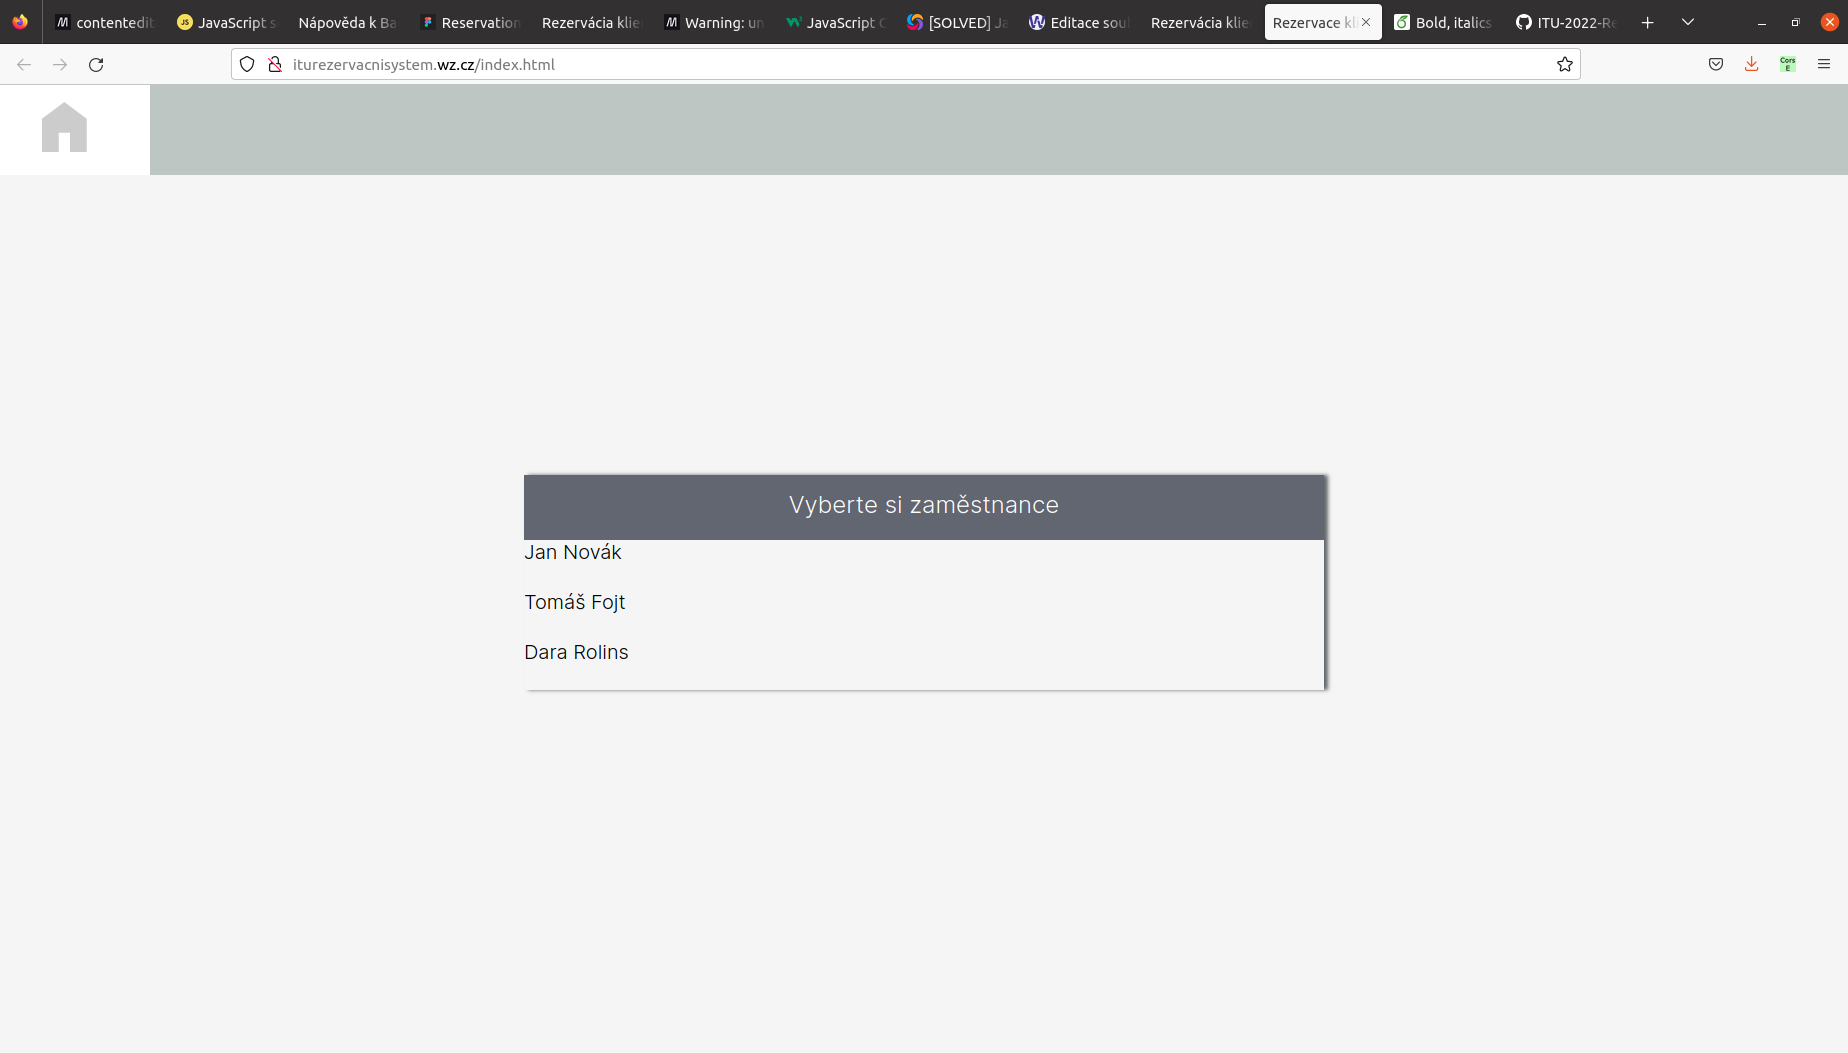
\includegraphics[width=.8\linewidth]{doc/latex/fig/implementation/client/step5.png}
        \caption{}
        \label{fig:step5}
    \end{subfigure}
    \begin{subfigure}{.5\textwidth}
        \centering
        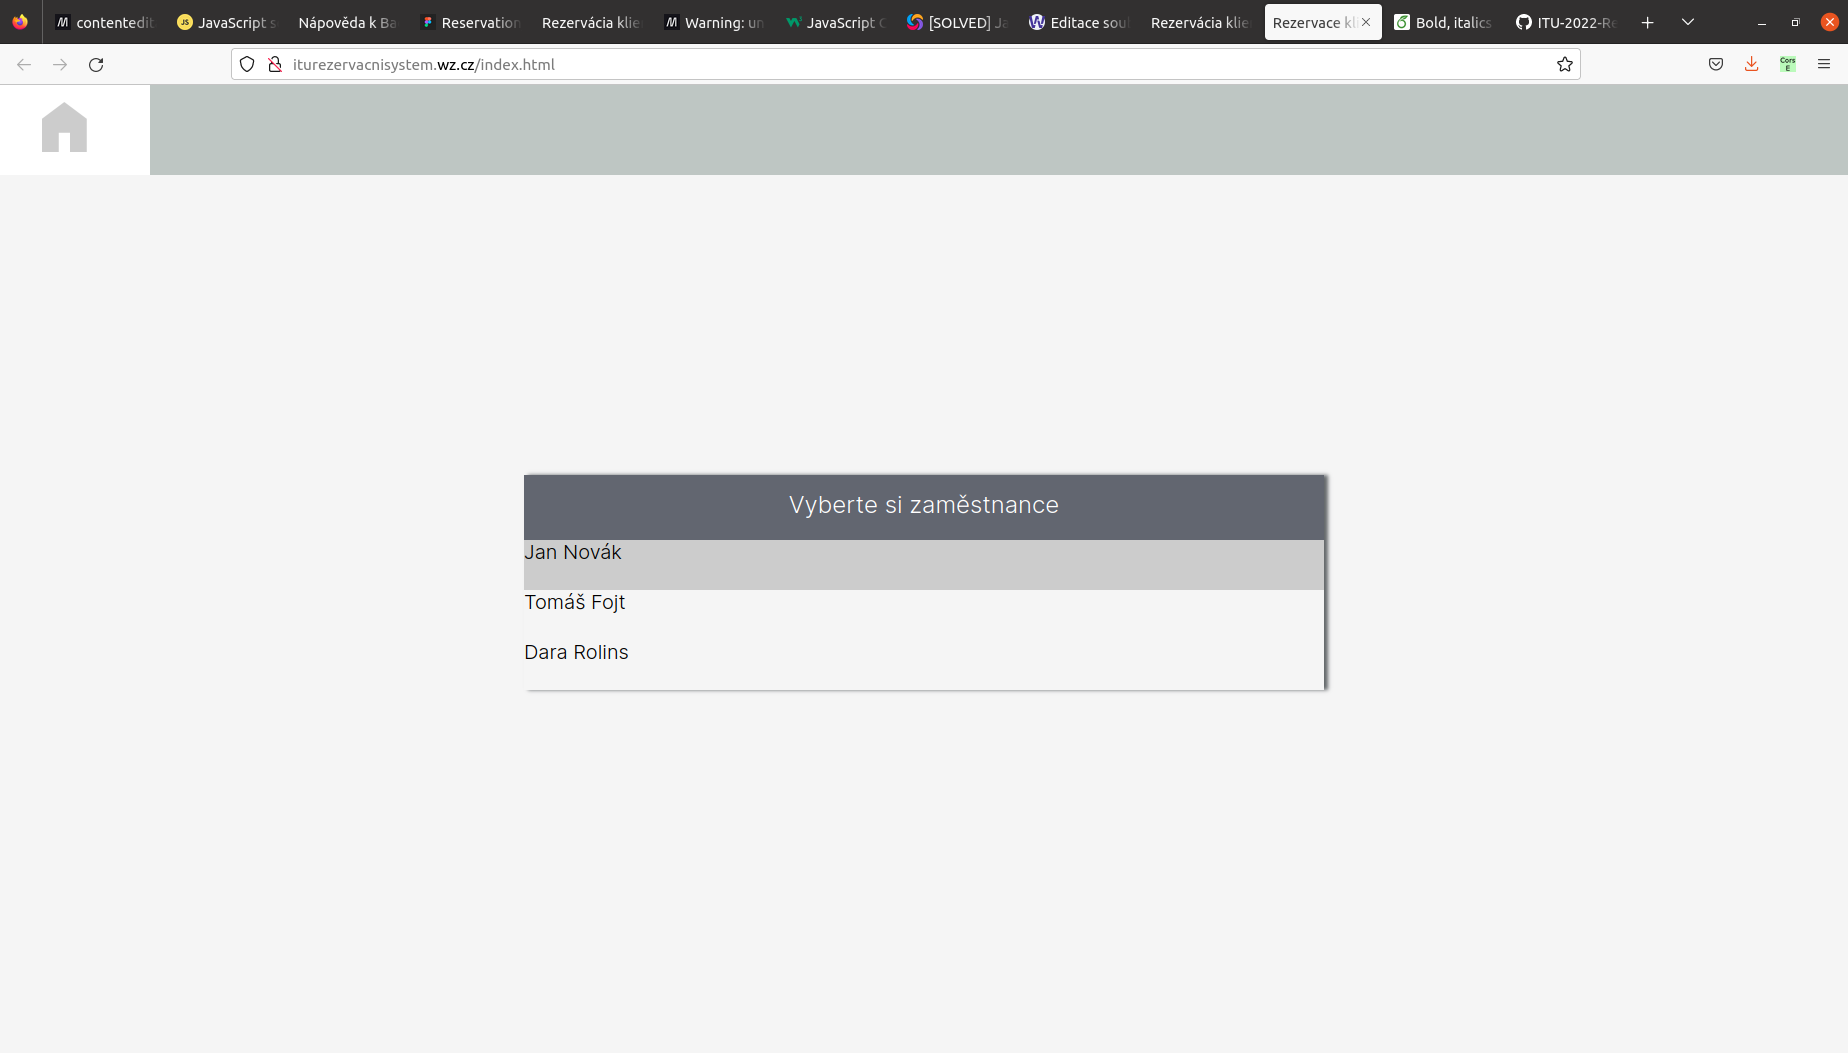
\includegraphics[width=.8\linewidth]{doc/latex/fig/implementation/client/step6.png}
        \caption{}
        \label{fig:step6}
    \end{subfigure}
    \caption{}
    \label{fig:steps3}
\end{figure}

\begin{figure}[h]
    \centering
    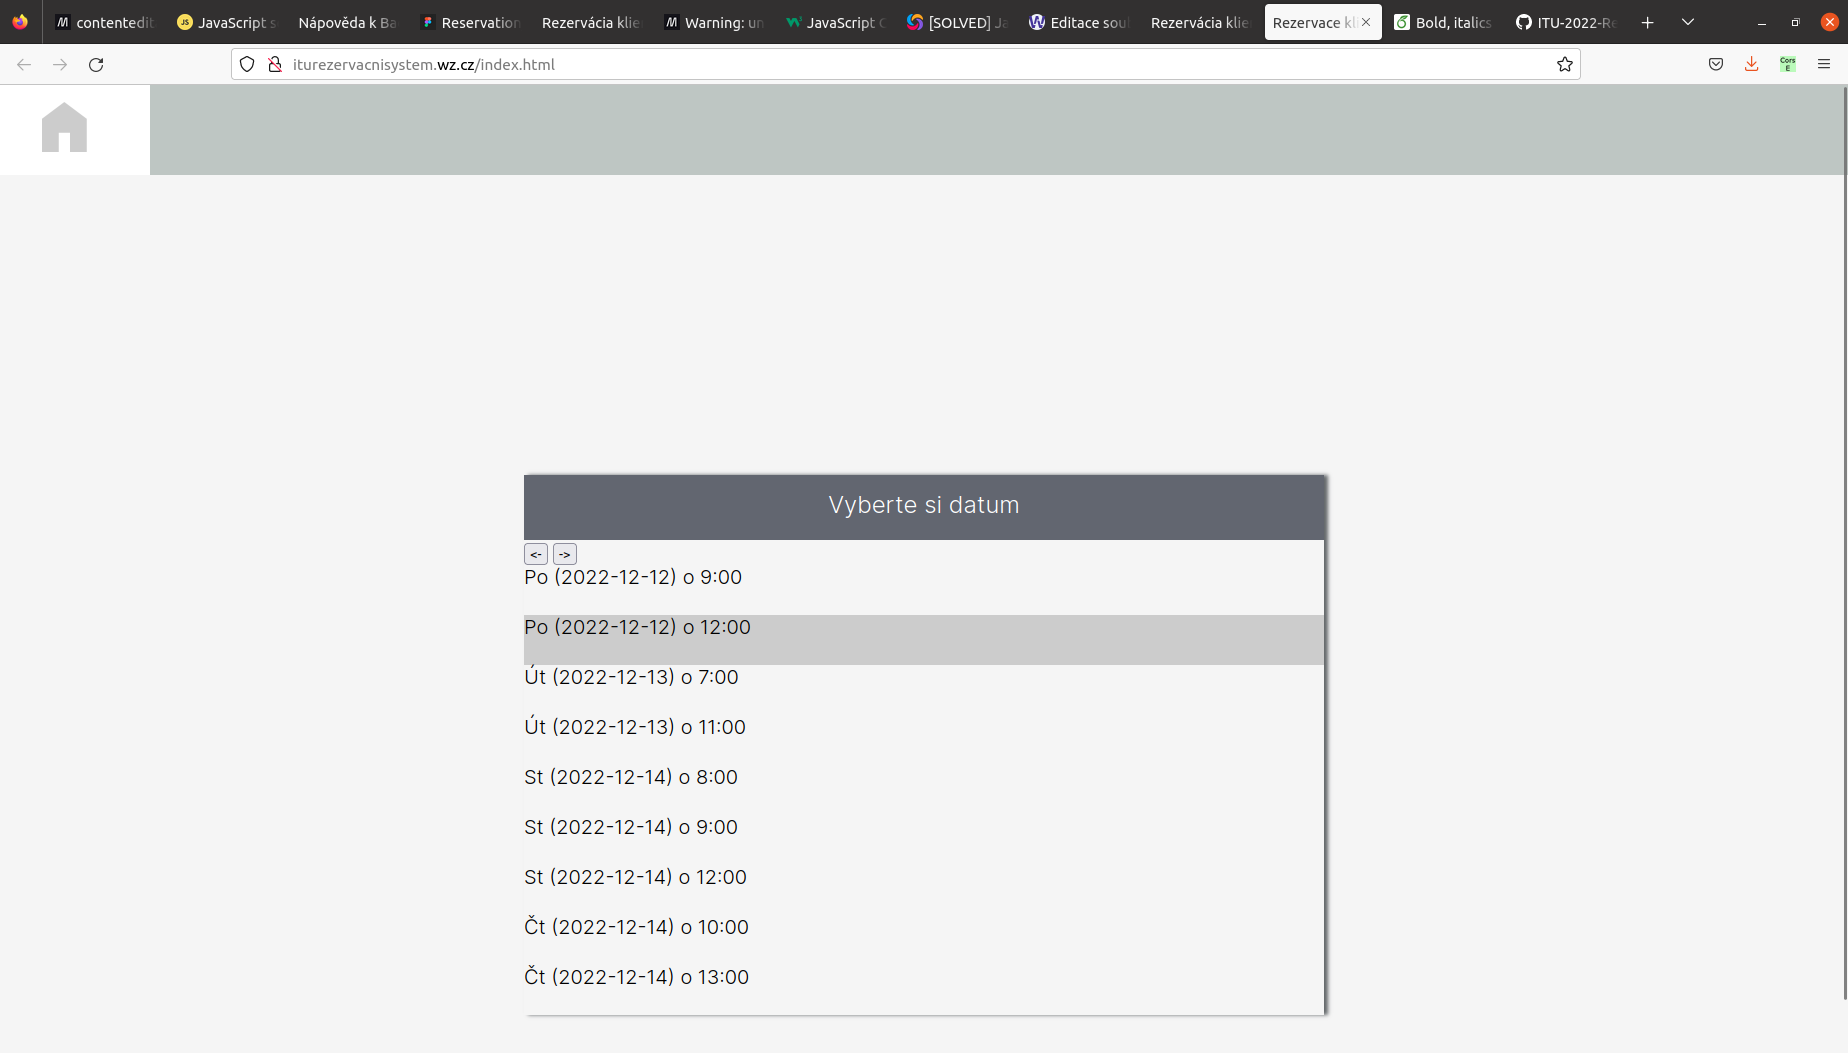
\includegraphics[width=.8\textwidth]{doc/latex/fig/implementation/client/step7.png}
    \caption{}
    \label{fig:step7}
\end{figure}

\newpage
